\documentclass[fleqn,usenatbib,useAMS]{mnras}

\usepackage{graphicx}	% Including figure files
\usepackage{amsmath}	% Advanced maths commands
\usepackage{amssymb}	% Extra maths symbols
\usepackage{multicol}        % Multi-column entries in tables
\usepackage{bm}		% Bold maths symbols, including upright Greek
\usepackage{pdflscape}	% Landscape pages
\newcommand{\kms}{\,km\,s$^{-1}$} % kilometres per second
\newcommand{\bibtex}{\textsc{Bib}\!\TeX} % bibtex. Not quite the correct typesetting, but close enough

\usepackage[T1]{fontenc}
\usepackage{ae,aecompl}


%\usepackage{newtxtext,newtxmath}

%\documentclass[fleqn,usenatbib]{mnras}
%\usepackage{newtxtext,newtxmath}
%\usepackage[T1]{fontenc}

\usepackage{bigints}    %larger integrals
\usepackage{units}
\usepackage{tabularx}
\usepackage{cleveref}
\crefformat{section}{\S#2#1#3} % see manual of cleveref, section 8.2.1
\crefformat{subsection}{\S#2#1#3}
\crefformat{subsubsection}{\S#2#1#3}
%%%%%%%%%%%%%%%%%%%%%%%%%%%%%%%%%%%%%%%%%%%%%%%%%%

\usepackage{ulem}
\usepackage[dvipsnames]{xcolor}
\newcommand{\mjv}{\textcolor{cyan}}
\newcommand{\edit}{\textcolor{red}}
\newcommand{\Referee}{\textcolor{red}}
%%%%%%%%%%%%%%%%%%%%%%%%%%%%%%%%%%%%%%%%%%%%%%%%%%

\newcommand{\be}{\begin{equation}}
\newcommand{\ee}{\end{equation}}
\newcommand{\ba}{\begin{eqnarray}}
\newcommand{\ea}{\end{eqnarray}}
\newcommand{\mperh}{\,h^{-1}\,{\rm Mpc}}
\newcommand{\hperm}{\,h\,{\rm Mpc}^{-1}}
\newcommand{\todo}[1]{{\em \textcolour{red}{ #1}}}
\newcommand{\lang}{\langle}
\newcommand{\ra}{\rangle}
\newcommand{\vc}{\bm{c}}
\newcommand{\va}{\bm{a}(z)}
\newcommand{\vb}{\bm{b}(z)}
\newcommand{\vCo}{\bm{C}_{\rm obs}}
\newcommand{\vCoi}{\bm{C}_{\rm obs}^{-1}}
\newcommand{\vCi}{\bm{C}_{\rm int}(z)}
\newcommand{\vCii}{\bm{C}_{\rm int}^{-1}(z)}
\newcommand{\vCt}{\bm{C}_{\rm tot}(z)}
\newcommand{\vCti}{\bm{C}_{\rm tot}^{-1}(z)}
\newcommand{\ep}{\epsilon}
\newcommand{\pars}{\vec{\theta}}
\newcommand{\dev}{\mathrm{d}}
\newcommand{\mstar}{h^{-1}M_\odot}
\newcommand{\mrefz}{m_{i, \mathrm{ref}}}
\newcommand{\mi}{m_{i}}
\newcommand{\dense}{\mathtt{dense}}
\newcommand{\lum}{\mathtt{luminous}}
\newcommand{\dk}{\boldsymbol{w}_{g}^{(k)}}
\newcommand{\dg}{\boldsymbol{\gamma}_{t}}
\newcommand{\dbar}{\overline{\boldsymbol{w}_{g}}}
\newcommand{\njk}{N_{\rm JK}}
\newcommand{\healpix}{\mathtt{HEALPIX}}

%%%%%%%%%%%%%%%%%%% TITLE PAGE %%%%%%%%%%%%%%%%%%%

\title[KiDS LRGs]{Clustering of red-sequence galaxies in the fourth data release of the Kilo Degree Survey}


\author[M. Vakili et al.]{
Mohammadjavad Vakili$^{1}$\thanks{E-mail: vakili@mail.strw.leidenuniv.nl}, KiDS Collaboration\\
% List of institutions
$^{1}$Leiden Observatory, Leiden University, Leiden, Netherlands
}

% These dates will be filled out by the publisher
\date{Accepted XXX. Received YYY; in original form ZZZ}

% Enter the current year, for the copyright statements etc.
\pubyear{2018}

% Don't change these lines
%FIXME 
%\hypersetup{draft}

\begin{document}
\label{firstpage}
\pagerange{\pageref{firstpage}--\pageref{lastpage}}
\maketitle

% Abstract of the paper
\begin{abstract}

We present a sample of luminous red-sequence galaxies for studying the large-scale structure in the Kilo-Degree Survey (KiDS). The selected galaxies are well-described by a red-sequence template, a data-driven model of the color-magnitude relation as a function of redshift. In this work, the red-sequence template is calibrated using the broad-band optical+NIR photometry of KiDS-VIKIING and the overlapping spectroscopic datasets.    
The selection process involves estimating the red-sequence redshifts, their corresponding uncertainties, assessment of the purity of the sample, and the redshift distributions in tomographic bins.

Then we inspect the correlation between the number density of these galaxies and the survey systematic properties such as varying depth. These systematic correlations are mitigated by generation of non-uniform random point catalogs using self organizing maps. Finally, we measure the angular two-point correlation function of these galaxies in tomographic bins and we provide theoretical fits to these measurements. 

\end{abstract}

% Select between one and six entries from the list of approved keywords.
% Don't make up new ones.
\begin{keywords}
galaxies: distances and redshifts, gravitational lensing: weak, methods: data analysis, methods: statistical
\end{keywords}
%\textbf{}\clearpage
%%%%%%%%%%%%%%%%%%%%%%%%%%%%%%%%%%%%%%%%%%%%%%%%%%

%%%%%%%%%%%%%%%%% BODY OF PAPER %%%%%%%%%%%%%%%%%%

\section{Introduction}

The Kilo Degree Survey (KiDS) is an optical galaxy survey primarily designed to map the large scale structure by studying the weak gravitational lensing of galaxies (\citealt{kuijken2015, kuijken2019}). This is done by measuring the correlation between the distortion of the shapes of distant galaxies (\citealt{hendrick2017,hendrik2018}). These correlations are then compared to the predictions of cosmological simulations to test cosmological models (\citealt{heymans2013,jee2016,hendrick2017,joudaki2017,troxel2017,joudaki2019, hikage2019}). 

However, the full constraining potential of weak lensing studies can only be realized through joint 
analysis of the cosmic shear of back ground galaxies and the positions of foreground galaxies with robust distance estimates. This involves measuring the correlation between the cosmic shear estimates of the background galaxies, the correlation between the positions of foreground galaxies, and eventually the cross-correlation between the cosmic shear of background galaxies and the positions of foreground galaxies (\citealt{cacciato2013, cosmolike, des_y1_cosmology, elvin2017, edo2018, prat2017}). 

The advantages of such combined analyses are two-folded: obtaining tighter constraints on cosmological parameters and the possible extensions to the standard model of cosmology, and providing a venue for mitigation of a range of observational and systematic uncertainties such as intrinsic alignments and the photometric redshift uncertainties (\citealt{edo2016, joudaki2018, sam2019}).

Following the work of \citet{vakili2019} we construct a galaxy sample with robust photometric redshifts by taking advantage of the properties of galaxies with old stellar populations. At any given redshift, the distribution of these galaxies in the colour-magnitude diagram follows a straight line --- with some intrinsic scatter --- known as the red-sequence ridge-line \citep[e.g.][]{bower1992,ellis1997,gladders1998,stanford1998}. Therefore, these galaxies are called the red-sequence galaxies. 

The redshift-dependent distribution of the red-sequence galaxies in the colour-magnitude diagram permits us to select these galaxies with the broad-band photometry of the imaging surveys (\citealt{gladders_yee2000,hao2009,redmap_sdss,rozo2016,elvin2017,oguri2018,vakili2019}). Th data-driven model of the color-magnitude relation of the red-sequence galaxies as a function of redshift is called the red-sequence template.

In this work, we select a set of red-sequence galaxies from the multi-band photometry of the KiDS DR4 (\citealt{kuijken2019}). 

The selected galaxies are well-described by the red-sequence template, which itself, is calibrated with a set of spectroscopic redshifts obtained by four spectroscopic datasets, including SDSS DR13 (\citealt{sdss_dr13}), GAMA (\citealt{driver2011}), 2dFLenS (\citealt{blake2016}), and the GAMA reanalysis of the redshifts in G10-COSMOS region (hereafter G10-COSMOS \citealt{davis2015}). Following the $\textsc{redMagiC}$ prescription (\citealt{rozo2016}), we impose a set of luminosity cuts and constant comoving densities, and we construct two samples of luminous red galaxies suitable for galaxy clustering and galaxy-galaxy lensing measurements. We call the sample with the lower (higher) luminosity threshold, the dense (luminous) sample.

The only difference between the method described in this work and the previous work of \citet{vakili2019} is the inclusion of the VIKING $Z$-band magnitudes in the red-sequence template. It is worth noting that while the $\textsc{redMagiC}$ algorithm relies on the redMapper \citealt{redmap_des} to calibrate the red-sequence template\footnote{Building the red-sequence template of the redMapper algorithm itself relies on spectroscopic data \citealt{redmap_sdss}}, we make use of the significant overlap of the KiDS DR4 data with external spectroscopic datasets. 

Furthermore, we make use of the VIKING $K_{\rm s}$-band magnitudes to investigate the purity of the selected samples with different luminosity thresholds. Given the purity of the samples and the variable depth of the survey, we choose the redshift reaches of the dense and the luminous samples. The redshift reach of each sample is chosen such that the sample remains nearly pure and nearly volume-limited below that redshift. Afterwards, we divide the galaxy sample into four tomographic redshift bins between 0.15 and 0.8, with the first three redshift bins comprising the dense galaxy sample and the last bin consisting of the galaxies in the luminous sample. 

Given that the galaxy clustering measures the probability, in excess of randoms, of finding pair of galaxies at a given angular or physical separation, accounting for the impact of survey properties on the galaxy density variations across the survey requires a careful treatment. The properties as well as the observing strategies of the galaxy surveys can influence the detection of galaxies as well as the selection process of any galaxy sample in the survey \citep[e.g.][]{alam2017,kwan2017,ross2017,elvin2017,crocce2019,kalus2019}. These properties include the variable depth of the survey in the multiple bandpasses, the seeing, etc. Furthermore, the on-sky galaxy density variations are susceptible to star density variations across the survey as well as the galactic extinction (\citealt{ignacio2018,rezaie2019}). 

In this investigation, we follow the newly developed technique based on self-organizing-maps (\citealt{johntson2019}) to produce sets of random points that ingest the correlation of galaxy number densities with the survey systematic properties. We demonstrate the performance of the random points in terms of mitigating the galaxy-survey systematic correlations. Lastly, we compute the two-point correlation function and assuming a linear galaxy bias model and a nonlinear matter power spectrum at fixed cosmology, we provide theoretical fits to the compute angular clustering measurements in different tomographic bins. 

This paper is structured as follows. The data, both photometric and spectroscopic, are described in Section~\ref{sec:data}. In Section~\ref{sec:selection} we discuss the sample selection and the photometric redshifts. We then present the galaxy-density systematic correlations, production of randoms, and the performance of randoms in Section~\ref{sec:systematic}. In Section~\ref{sec:clustering} we present the computed two-point correlation functions as well as the theoretical fits.
Finally, we summarize and conclude in Section~\ref{sec:summary}. 

%Note that calculating the comoving densities and distances requires specifying a cosmology. In this work, we assume a flat $\Lambda$CDM cosmology with $\Omega_{m} = 0.3$ and $h=1.0$ \footnote{This is the convention used by \citet{redmap_sdss} in constructing the SDSS redMaPPer catalogue.}. All distances (comoving densities) are quoted in units of $h^{-1}\; \mathrm{Mpc}$ ($h^{3} \; \mathrm{Mpc}^{-3}$) respectively. Also note that the luminosity ratios used for selection of the red galaxies are not sensitive to the choice of $h$ and in this work and we always work with luminosity ratios. Whenever magnitudes are used, they will be provided in the AB system.

\section{Data}\label{sec:data}

\subsection{KiDS photometric data}\label{sec:kids}
The Kilo-degree Survey (KiDS, \citealt{kids}) is a wide 
imaging survey conducted with the OmegaCAM camera (\citealt{omegacam}) which is mounted on the VLT Survey Telescope (\citealt{vst}). This survey uses four broad-band filters ($ugri$) in the optical wavelengths. KiDS has targeted approximately 1350 deg$^2$ of the sky in two regions, one on the celestial equator and the other one in the South Galactic cap. 

KiDS broadband photometry in the optical is supplemented by the VISTA Kilo degree Infrared Galaxy (VIKING) survey (\citealt{irwin2004,lewis2010,Edge2013,Gonz2018}). The VIKING observations of nearly the same regions with the near infrared filters $ZYJHK_{s}$ significantly increase the wavelength coverage of KiDS, turning the KiDS dataset into a unique wide-field optical+NIR catalog suitable for cosmological analysis.

In this work we use the fourth KiDS data release (KiDS DR4 \citealt{kuijken2019}) which covers $1006$ deg$^{2}$ of the sky in 1006 tiles superseding the 440 tiles released in KiDS DR3 (\citealt{kids_dr3}). Reduction of the $ugri$ images was performed with the AstroWise pipeline (\citealt{omegacam}).  


The achieved 5$\sigma$ limiting AB magnitudes of the survey are 24.3, 25.1, 24.9, 23.8 in $2$ arcsec apertures in the $ugri$ bands respectively. For a thorough description of the KiDS data processing, we refer the readers to the data release paper (\citealt{kuijken2019}). 

The KiDS database includes magnitudes in the $r$-band derived by SExtractor (\citealt{sextractor}) such as \texttt{ISO} and \texttt{AUTO}. These magnitudes are determined directly from images with a variety of PSF values, they are therefore not optimal for our purposes where colours independent of such variations are needed. The KiDS data reduction involves however a post-processing procedure in which Gaussian Aperture and PSF (GAaP,~\citealt{gaap}) magnitudes are derived (\citealt{kuijken2015}). This procedure is performed in the following way. First, the PSF is homogenized across each individual coadd. Afterwards, a Gaussian-weighted aperture is used to measure the photometry. The size and shape of the aperture is determined by the object's length of the major axis, its length of the minor axis, and its orientation, all measured in the $r$-band. This procedure provides a set of magnitudes for all filters. 

The magnitudes used in this work are the zeropoint-calibrated and foreground dust extinction-corrected magnitudes\footnote{In the final catalogue and for each band, the zeropoint offsets ($\mathtt{ZPT}_{-}\mathtt{offset}_{-}\mathtt{band}$) and the Galactic extinction corrections ($\mathtt{EXT}_{-}\mathtt{SFD}_{-}\mathtt{band}$) based on \citet{schlegel98} are provided in separate columns.} 
denoted by $\; \mathtt{Mag}_{-}\mathtt{type}_{-}\mathtt{band}_{-}\mathtt{calib}$. 
In this notation, $\mathtt{calib}$ refers to the zeropoint-calibrated and extiction corrected magnitudes. $\mathtt{type}$ refers to the type of the magnitude, such as GAaP, $\mathtt{AUTO}$, or $\mathtt{ISO}$ magnitudes. Furthermore, $\mathtt{band}$ refers to the photometric band under consideration (i.e. $ugri$). The default magnitudes in KiDS are GAaP magnitudes, which were designed to provide accurate colours but underestimate total fluxes of large galaxies. Total fluxes are, however, needed in our LRG selection procedure to derive luminosities (see section~\ref{sec:overview}). Therefore, whenever galaxy fluxes are needed, we use $\mathtt{Mag}_{-}\mathtt{AUTO}_{-}\mathtt{band}_{-}\mathtt{calib}$ in our red-sequence modelling. 

For our choice of colour, GAaP colours are used as they have less scatter and bias than the colours derived from the $\mathtt{Mag}_{-}\mathtt{AUTO}_{-}\mathtt{band}_{-}\mathtt{calib}$ magnitudes. For the rest of this paper, we work with the calibrated $\mathtt{AUTO}$ $r$-band magnitude and GAaP colours. We emphasize that the GAaP procedure is intended to derive more accurate and less noisy estimates of colours for objects. In other words, the GAaP colours are less noisy than the colours estimated from the calibrated $\mathtt{AUTO}$ magnitudes ($\mathtt{Mag}_{-}\mathtt{AUTO}_{-}\mathtt{band}_{-}\mathtt{calib}$). We refer the readers to \citet{kuijken2015} and \citet{kids_dr3} for a more detailed discussion of the derivation of GAaP colours.

The nine-band photometric catalog is supplemented by a mask information
which removes the satellite tracks and other imaging artefacts such as stellar halos from the images. In KiDS DR4, the masking is carried out at the sub-exposure level, increasing the effective area of the coadd images.

\subsection{Spectroscopic data}\label{sec:spec}

In~\citet{vakili2019} we made use of the spectroscopic data of SDSS DR13, GAMA, and 2dFLenS. 
In addition to these data, we also take advantage of the KiDS deep field observation of the cosmos region, which overlaps with a number of spectroscopic campaigns such as zCOSMOS. 
In the COSMOS field we utilize the GAMA-G10 COSMOS spectrocopic data, which encompasses a wider magnitude range, albeit a much narrower area than the other spectroscopic data considered in this work. In what follows, we describe the spectroscopic datasets.

In this work, we exploit the overlap between the KiDS catalogue and a number of spectroscopic datasets. These datasets are used for the training and assessing the performance of the red-sequence template in selection and redshift estimation of LRGs.  
This procedure is explained in detail in our previous work (\citealt{vakili2019}). 

In addition to the datasets that we utilized in \citet{vakili2019}, we make use of the data
and it is applied to the overlap between the KiDS photometry and spectroscopic catalogues of galaxies in GAMA (\citealt{driver2011}) and SDSS DR13 (\citealt{sdss_dr13}). Later, for testing the performance of the redshifts estimated for the selected LRGs in section~\ref{sec:performance} we make use of the overlap between KiDS and the spectroscopic redshifts from SDSS, GAMA, as well as 2dFLenS (\citealt{blake2016}).
In what follows in the rest of this section, we provide a brief description of these spectroscopic catalogues.

We note that in general the spectroscopic samples such as those used here are systematically  brighter than the photometric data from which we will be selecting the LRGs. This means that bright galaxies are oversampled in the calibration data with respect to the faint end. However, this is not an issue for the LRG selection procedure of Sec.~\ref{sec:methodology}: what is needed is to have red spectroscopic galaxies to calibrate the red sequence template (colour-magnitude relation), which is approximately a straight line at each redshift. Consequently, one can use a relatively bright spectroscopic sample to estimate the colour-magnitude relation for fainter red galaxies.

The undersampling of the faint galaxies by overlapping spectroscopic data will be more of a problem for robust evaluation of photo-$z$ performance: at higher redshifts, the difference in average brightness between the full sample and the sample with spectroscopy is more significant than at the low-redshift, bright end, so the direct spec-$z$ -- photo-$z$ comparison may be indicating better performance than it actually is. We note however that the photo-$z$ error -- observational systematic trend presented in Sec.~\ref{sec:sys} will be still valid.

\subsubsection{GAMA}
Galaxy And Mass Assembly (GAMA,~\citealt{driver2011}) is a spectroscopic survey  which used the AAOmega spectrograph mounted on the Anglo-Australian Telescope. This survey spans five fields: G09, G12 and G15 on the celestial equators, and G02 and G23 on the Southern Galactic Cap. The only GAMA field outside the KiDS DR3 footprint is G02. The magnitude limited sample of GAMA is nearly complete down to $r=19.8$ mag for galaxies in the equatorial fields and down to $i=19.2$ mag for galaxies in the G23 region (\citealt{likse2015}). The GAMA spectra in the four fields that overlap with KiDS amount to a total of $\sim 230,000$ KiDS objects with high-quality spectroscopic redshifts with $\langle z \rangle = 0.23$. 

\subsubsection{SDSS}

The Sloan Digital Sky Survey (SDSS, \citealt{york2000}) is a photometric and spectroscopic survey of $14,555$ deg$^2$ of the sky encompassing more than one third of the celestial sphere using a dedicated 2.5-m telescope (\citealt{gunn2006}). In particular, we make use of the spectroscopic dataset from the Data Release 13 (DR13, \citealt{sdss_dr13}) of the SDSS-IV project. We only use objects with class `GALAXY'. 

The overlap between SDSS and KiDS in the equatorial fields above $\delta =-3$ ($\delta$ denotes the declination of objects on the sky) gives us $\sim 99252$ SDSS spectroscopic galaxies with KiDS photometry. However those with $r<19.8$ are mostly included in GAMA, and after removing the latter we are left with nearly $43,000$ unique SDSS spectroscopic galaxies with KiDS photometry. 

The SDSS-matched KiDS galaxies (after removing the overlap with GAMA) span higher redshifts than the GAMA-matched KiDS objects. This sample of galaxies mostly encompasses LRGs that are observed in the Baryonic Oscillation Spectroscopic Survey (BOSS, \citealt{dawson2013}) and the extended BOSS (eBOSS, \citealt{dawson2016}). This makes them ideal candidates for seed galaxies needed to estimate the red-sequence template as we seek to select galaxies that populate the same volume in the colour space as the SDSS LRGs do. 

\subsubsection{2dFLenS}
The 2-degree Field Lensing Survey (2dFLenS, \citealt{blake2016}) is a spectroscopic survey performed at the Australian Astronomical Observatory covering an area of 731 deg$^2$. By expanding the overlap with the KiDS field in the southern galactic cap, this survey aims to provide a dataset suitable for joint clustering and lensing analyses (\citealt{amon2018b,joudaki2018}), photometric redshift calibration (\citealt{johnson2017,wolf2017,kids_annz}), and lensing systematic tests (\citealt{amon2018a}).

In KiDS DR3 there are nearly $37461$ galaxies with 2dFLenS spectra. After excluding the galaxies in common with GAMA and SDSS, we have approximately $9,000$ unique 2dFLenS galaxies with KiDS photometry.

\subsubsection{GAMA-G10}

the Galaxy And Mass Assembly (GAMA) 10$^{\rm h}$ region (G10) (hereafter GAMA-G10) targets the data in the Cosmic Evolution Survey region (COSMOS). The GAMA-G10 consists of a curation and verification of approximately 16$k$ redshifts of bright galaxies in the COSMOS region (\citealt{davis2017}). Creation of this bright galaxy sample does not involve any target selection. All the 1$d$ and the 2$d$ spectra were process by the GAMA pipeline and were manually checked. Overall, the redshifts in this sample of bright galaxies are believed to be more robust than the redshifts obtained by the rest of the spectroscopic campaigns targeting the cosmos field \citep[e.g.][]{lily2009}.

\section{Sample selection}\label{sec:selection}

Several aspects of the selection procedure in this work are simillar to what has been outlined  in Vakili2019.  The main differences are the following. We include the VIKING $Z$ band in the red-sequence temlpate. In principle, one can also include the rest of the $YJHK_{\rm s}$ bandpasses of VIKING in the red-sequence modelling. However, we decided to exclude those bandpasses in the modelling as they would increase the computational cost of the following steps: $(i)$ selection of a set of seed galaxies for estimating the parameters of the red-sequence template, and eventually computing the conditional probability of color conditioned of the redsfhit and magnitudes of all the objects in the survey. 

As we discussed in Section~\ref{sec:data}, we make use the apparent AUTO magnitude in the $r$-band which is provided in KiDS DR4  as $\mathtt{MAG \underscore AUTO}$. The AUTO magnitude quantities are not provided in the rest of the KiDS-VIKING bandpasses. As discussed in Section~\ref{sec:data}. We make use of the GAaP $\{u-g,g-r,r-i,i-Z\}$ colors, which provide a more precise proxy for the colors of galaxies (\citealt{kuijken2019}). After evaluating $p(\boldsymbol{c}|m,z)$ and the red-sequence chi-squared $\chi^{2}_{\rm red}$, we proceed in a similar fashion as described in detail in \citet{rozo2016, vakili2019}. We construct two luminosity-threshold samples: the dense sample with $L>0.5 L_{\star}$ and a luminous sample with $L>L_{\star}$. 

In order to assess the purity of the two samples in the color space, we investigate the redshift-dependent distribution of galaxies in the $(r-Z, r-K_{s})$ space. In Figure~\ref{fig:star_galaxy_I}, we show the distribution of red-sequence galaxies and stars\footnote{selected from KiDS DR4 using $\mathtt{SG\underscore{}FLAG}= 0$} in this two-dimensional color space.  As apparent on the left panel of Figure~\ref{fig:star_galaxy_I}, the distribution of the colors of galaxies in the dense sample has significant overlap with the distribution of the colors of high confidence stars for $z>0.6$. On the other hand, there is more clear distinction between the color distribution of the luminous galaxies and that of the high confidence stars. 

\section{Survey systematics}\label{sec:systematic}

We consider a range of photometric systematic with on-sky variations that can impact the variations of galaxy number densities in our selection of LRGs in KiDS DR4. In total we consider 13 survey properties that we further pixellize using $\healpix$. We produce the $\healpix$ map of these properties with $n_{\rm side} = 256$. Moreover, we consider the galactic extinction in the $r$-band, and the star number density in the survey footprint. In what follows, we list the set of systematic properties considered in our investigation:

\begin{itemize}

  \item \textbf{Limiting magnitudes in 9 band}: The limitting GAaP magnitude attributes are provided in DR4 as $\mathtt{MAG}\textunderscore{}\mathtt{LIM}\textunderscore{} \mathtt{band}$, where $\mathtt{band} = \{u,g,r,i,z,H,Y,J,K_{\rm s}\}$. This limitting magnitudes are measured for the optimal value of the minimum aperture setting $\mathtt{MIN}\textunderscore{}\mathtt{APER}$ in GAaP photometry. In each band, the limiting GAaP magnitudes correspond to the 1-$\sigma$ flux errors. 
  
  \item \textbf{PSF FWHM in the $r$-band}: the KiDS seeing FWHM in the $r$-band measured in units of arcseconds. The PSF FWHM is calculated using the follwoing catalog entries: $\mathtt{PSFe1}$, $\mathtt{PSFe2}$, and $\mathtt{PSF \textunderscore{} Strehl \textunderscore{} ratio}$.
    \item \textbf{PSF ellipticity in the $r$-band}: the KiDS PSF ellipticity in the $r$-band. As discussed in \citet{kuijken2019}, both PSF ellipticity and the PSF FWHM in the $r$-band are small, allowing for benign imaging condition in the $r$-band which is used as the detection band in the KiDS photyometry pipeline. 
    The PSF ellipticity quantity is computed from the $\mathtt{PSFe1}$, $\mathtt{PSFe2}$
  \item \textbf{Detection threshold above background}: This quantity is measured in units of counts and it is provided in the single-band source list as $\mathtt{THRESHOLD}$. 
  \item \textbf{Background count in the THELI images}: The background counts at the centroid positions of the objects in the THELI-processed $r$-band detection images. In KiDS DR4, the background count is provided as $\mathtt{BACKGROUND}$. Note that the THELI processed detection images are background subtracted. The $\mathtt{BACKGROUND}$ parameter simply returns the value of the residual sky background at the positions of 
  objects.
  \item \textbf{Galactic dust extinction in the $r$-band}: This quantity is provided as $\mathtt{EXTINCTION\underscore{}r}$ in the nine-band catalog of KiDS DR4. The galactic extinction in the other bands are simply given by scaling of the extinction in the $r$-band.   
  \item \textbf{Star number density}: We determine the the stellar density from the pixellized number density map of bright stars in the second data release of GAIA (GAIA DR2). This is done by taking the GAIA stars with the $G$-band magnitude between 12 and 17. This is the magnitude range in which the GAIA DR2 G-band is complete (\citealt{gaia0,gaia1}). Note that only GAIA DR2 stars that lie in the KiDS 9bandnoAWr mask are considered in the number density map making process. It is worth noting that a number of parameters in the KiDS DR4 catalog are dedicated to star-galaxy separation. These include the $\mathtt{CLASS\textunderscore{}STAR}$
 parameter which is an output of the source extractor software, the $\mathtt{SG2DPHOT}$ parameter which is an internal KiDS star-galaxy classifier \citep[e.g.][]{kids_dr3, radovich2017}, and lastly the $\mathtt{SG\textunderscore{}FLAG}$ parameter which is derived based on an estimate of the size-peakiness relation of objects. Note that we have already excluded objects in our sample that are classified as high confidence stars according to the parameters $\mathtt{SG2DPHOT}$ and $\mathtt{SG\textunderscore{} FLAG}$. However, in order to reduce any impact of possible imperfections in the star-galaxy classification on our systematic tests, we decide to use a systematic map constructed from an external GAIA DR2 catalog with a pure and compete sample of stars. 
 
\end{itemize}

It is important to note that the systematic parameters considered in our investigation are not uncorrelated, an effect that may stem from the various survey strategies and observing conditions. 
Figure [fignum] demonstrates the correlation between various systematic parameters in the survey. 
For instance, there is a strong correlation between the limiting magnitude in the u band and the the star number density. 


\section{Galaxy Clustering}\label{sec:clustering}
\subsection{Theory}

Assuming a local linear galaxy bias, the galaxy overdensity $\delta_g$ can be related to the matter overdensity $\delta_m$ through a linear relation: $\delta_g = b_g \delta_m$, where the parameter $b_g$ is the linear bias parameter. Such assumption is expected to hold on sufficiently large scales \citep[e.g.][]{dvornik2018}, whereas on small scales, the nonlinear structure formation is best described by the more sophisticated halo model \citep[e.g. ][]{hand2017,vakili_hahn}.

For a given set of sample of galaxies with a linear bias parameter $b_g$ and redshift distribution of $n_g(z)$, and a nonlinear matter power-spectrum $P_{\delta}(k,z)$, one can predict the angular clustering of the galaxy sample.

\begin{eqnarray}
w_{g}(\theta) &=& b_g^2 \int \frac{l dl}{2\pi}J_{0}(l\theta)  \nonumber \\ 
            &\times& \int d\chi_{\rm cov} \Big[\frac{n_{g}(z)dz/d\chi_{\rm cov}}{\chi_{\rm cov}}\Big]^{2}P_{\rm NL}\Big(k = \frac{l+1/2}{\chi_{\rm cov}}; \; z\Big),                  
\label{eq:clustering_theory}
\end{eqnarray}
where $\chi_{\rm cov}$ is the comoving distance with a redshift dependence that is itself depend on the choice of cosmology. The term $P_{NL}$ is the analytical nonlinear power spectrum which can be calculated using different recipes  \citep[e.g. ][]{takahashi2012, emu2014,mead2015, smith2019}.

In practice, we calculate the theoretical prediction (\ref{eq:clustering_theory}) for all four tomographic bins in our galaxy sample, each with their corresponding linear bias parameter $b^{(i)}_{g}$ and redshift distribution $n^{(i)}_{g}(z)$, where $i\in {1,2,3,4}$ corresponds to the tomographic bins defined in Section~\ref{sec:selection}.

Assuming a fixed cosmology, we estimate the linear bias parameters $\{b^{(i)}_{g}\}_{i=1}^{4}$ by fitting the theoretical prediction (\ref{eq:clustering_theory}) to the angular clustering measurements provided in Section~\ref{sec:measurement}. It is important to note that one major source of systematic in this theoretical prediction is the uncertainty on the mean of the redshift distributions $\{n_{g}^{(i)}(z)\}_{i=1}^{4}$. In order to mitigate the impact of such systematic, we assume that the estimated redshift distribution at each tomographic bin $n_{g}^{(i)}(z)$ is effectively given by shifting the unbiased redshift distribution $n_{g, \rm true}^{(i)}(z - \delta z^{(i)})$, where the $\delta z^{(i)}$ parameter is the on the mean of the redshift distribution at the $i$-th tomographic bin. In Section~\ref{sec:selection} we have estimated these redshift uncertainties. While constraining the galaxy bias parameters, we marginalize over the individual redshift uncertainties. 

\subsection{Clustering measurements}\label{sec:measurement}

Galaxy 2PCF is the probability in excess of random of finding two-pairs of galaxies within a given angular or physical separation. Given that we do not know the exact redshifts of the galaxies, we focus on computing the angular 2PCF which can be obtained by performing pair-counts in angular bins. The angular clustering can be measured using the Landy-Szalay estimator (\citealt{landy}):
\begin{equation}
    \hat{w}(\theta) = \frac{DD-2DR+RR}{RR},
\label{eq:landy}
\end{equation}
where $DD$ denotes the number of galaxy pairs within an angular separation bin centered at $\theta$, $DR$ denotes the number galaxy-random pairs, and $RR$ denotes the number of random pairs. 

As discussed in Section~\ref{sec:systematic}, we have generated an organized random catalog for each galaxy sample which belongs to the tomographic bins defined in Section~\ref{sec:selection}. These organized random catalogs are designed such that they mimic the variations in the galaxy density that are due to on-sky variation of the survey systematic properties. In what follows in this section we compute the angular 2PCF for two sets of random points: one for the uniform randoms, and one for the organized randoms.

Figure~\ref{fig:xi} shows the angular clustering measurements of LRG's at 4 tomographic bins, with the first three bins encompassing the galaxies in the dense sample and the last bin ($0.6<z<0.8$) encompassing the galaxies in the luminous sample. The clustering signal estimated using the uniform randoms is shown by the orange data points and the signal estimated using the organized randoms is shown by the blue data points. 

We estimate the measurement uncertainties using the jackknife resampling method (\citealt{norberg2009,oliver2016,singh2017,shirasaki2017}). 
In the jackknife method, the survey footprint is first divided into $N_{\mathrm{JK}}$ jackknife subregions of approximately equal area. 
Then for each subregion $k\in\{1,...,N_{\mathrm{JK}}\}$, the clustering data vector $\boldsymbol{w}_{g}^{(k)} = \langle w^{(k)}_{g}\rangle$ is measured by cutting out the $k$-th subregion and estimating the clustering signal of the rest of the survey footprint. Note that $\boldsymbol{w}_{g}^{(k)}$ is a vector which contains the 2PCF in all angular bins considered in this study. The jackknife estimator of the covariance matrix is then given by:
\be 
C_{\rm JK} = \frac{\njk - 1}{\njk}\sum_{k=1}^{\njk}\big(\dk-\dbar\big)^{T}\big(\dk-\dbar\big), 
\label{eq:jk}
\ee
where $\dbar$ is the mean of all $\boldsymbol{w}_{g}^{(k)}$ vectors. 


\subsection{Galaxy bias}
\section{Summary}\label{sec:summary} 





\section*{Acknowledgements}


\begin{figure*}
\begin{tabular}{cc}
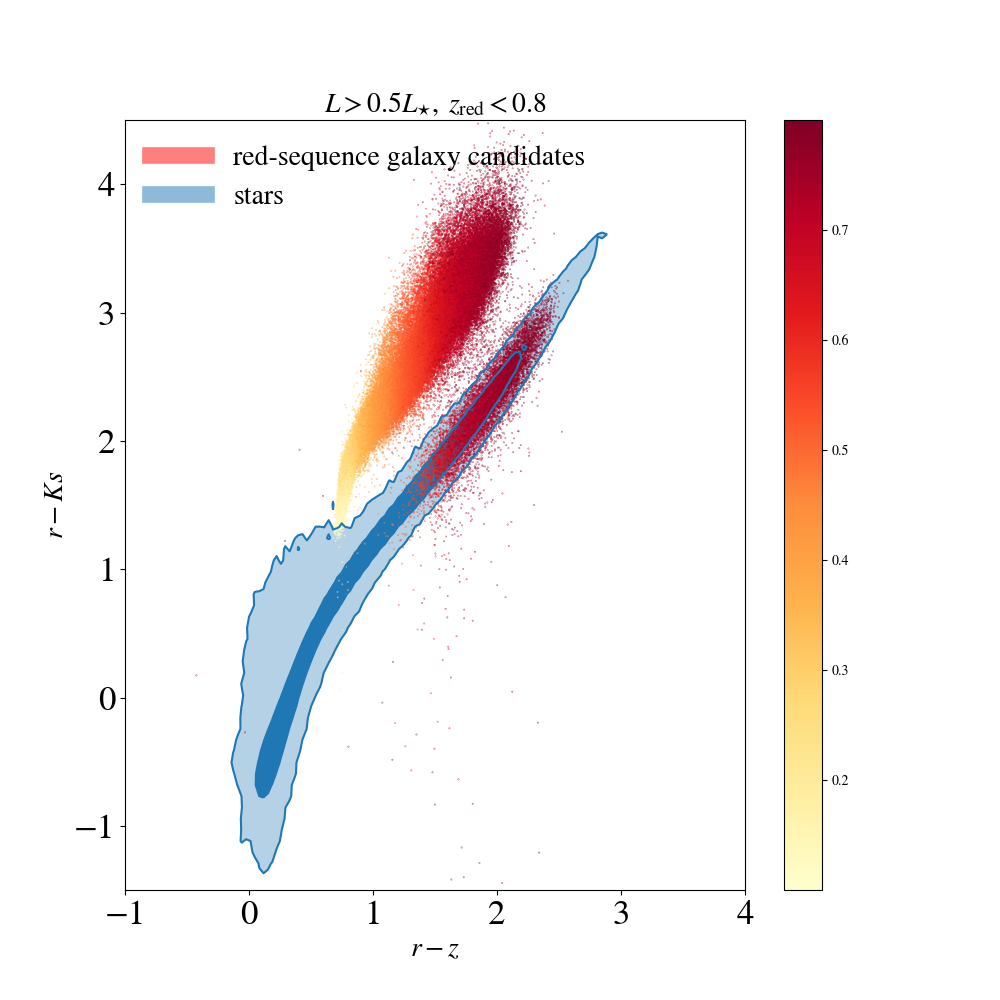
\includegraphics[width=0.5\textwidth]{figures_tmp/red_vs_star_dense.png}
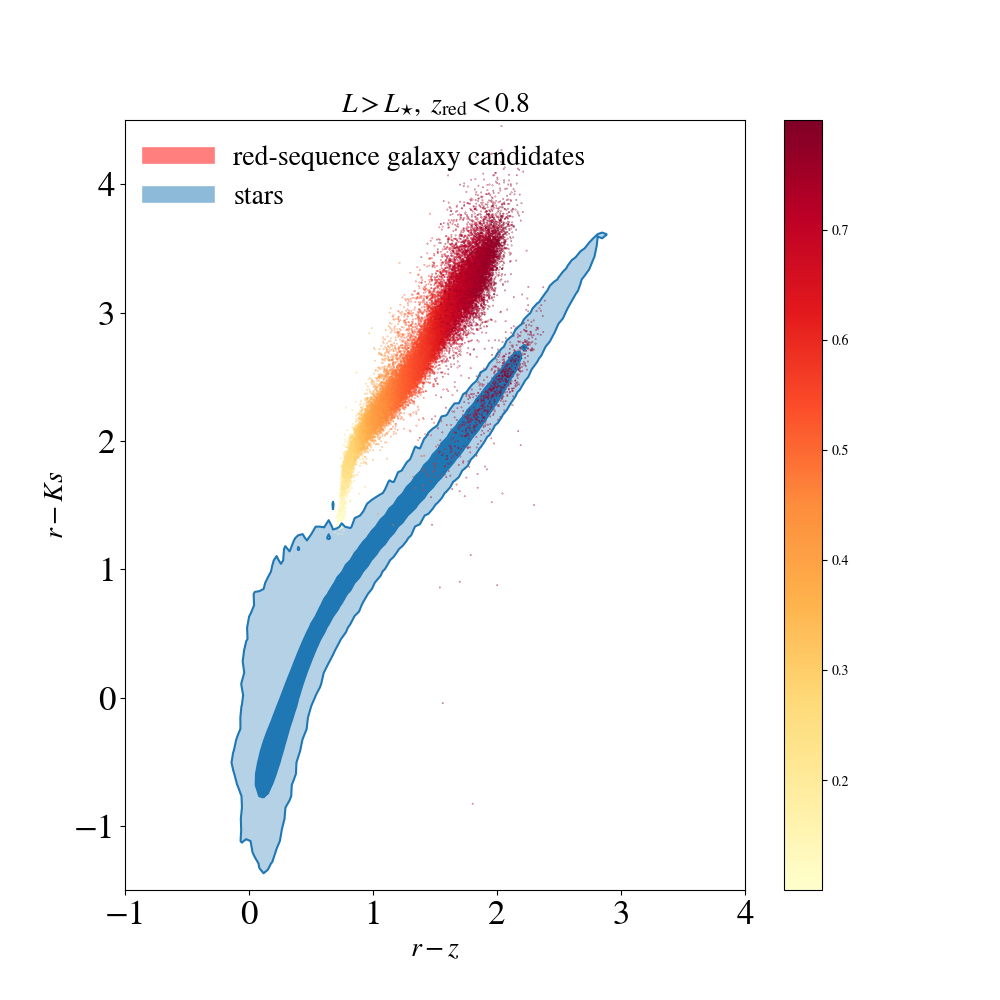
\includegraphics[width=0.5\textwidth]{figures_tmp/red_vs_star_lum.png}
\end{tabular}
\caption{\label{fig:star_galaxy_I} Demonstration of the use of optical+NIR colors for identification of likely stellar objects amongst the red-sequence galaxy candidate. Right Panel: At redshifts above $z_{\rm red}>0.4$ red-sequence galaxies (shown in red) and high confidence stars (shown in blue) reside in separated regions of the two-dimensional $(r-K_{\rm s}) \times (r-z)$ colors. Shown in pink dashed line is the support vector machine prediction of a boundary line between the two classes. The red-sequence candidates falling below the predicted boundary are marked by open circle and thus masked as likely stellar objects in the final catalog. Left Panel: Purity fraction of the dense  (green dashed line) and the luminous (orange dashed line) samples defined as the stellar contamination fraction subtracted from unity.} 
\end{figure*}


\begin{figure*}
\begin{tabular}{cc}
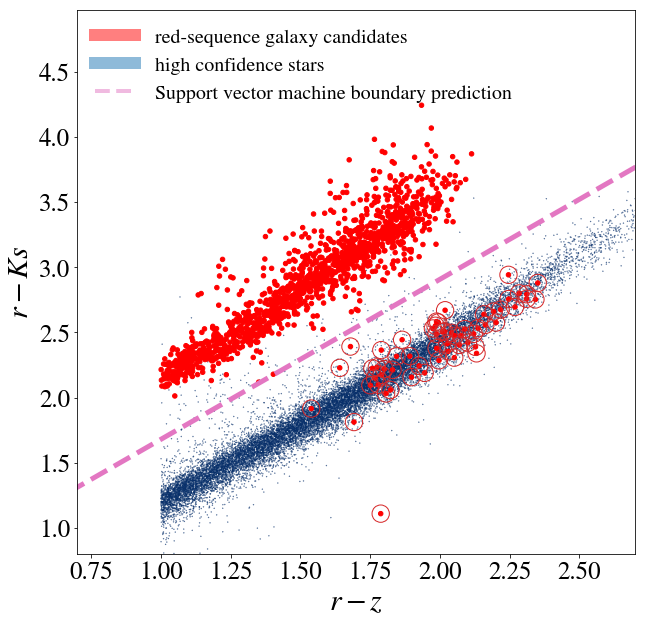
\includegraphics[width=0.5\textwidth]{figures_tmp/stars_SVM_lum.png}
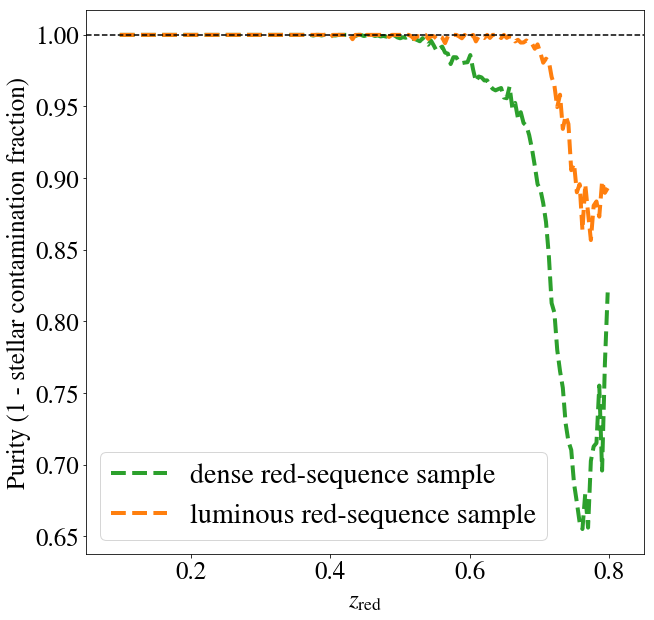
\includegraphics[width=0.5\textwidth]{figures_tmp/purity}
\end{tabular}
\caption{\label{fig:star_galaxy_II} Demonstration of the use of optical+NIR colors for identification of likely stellar objects amongst the red-sequence galaxy candidate. Right Panel: At redshifts above $z_{\rm red}>0.4$ red-sequence galaxies (shown in red) and high confidence stars (shown in blue) reside in separated regions of the two-dimensional $(r-K_{\rm s}) \times (r-z)$ colors. Shown in pink dashed line is the support vector machine prediction of a boundary line between the two classes. The red-sequence candidates falling below the predicted boundary are marked by open circle and thus masked as likely stellar objects in the final catalog. Left Panel: Purity fraction of the dense  (green dashed line) and the luminous (orange dashed line) samples defined as the stellar contamination fraction subtracted from unity.} 
\end{figure*}



\begin{figure*}
 
 \begin{tabular}{cc}
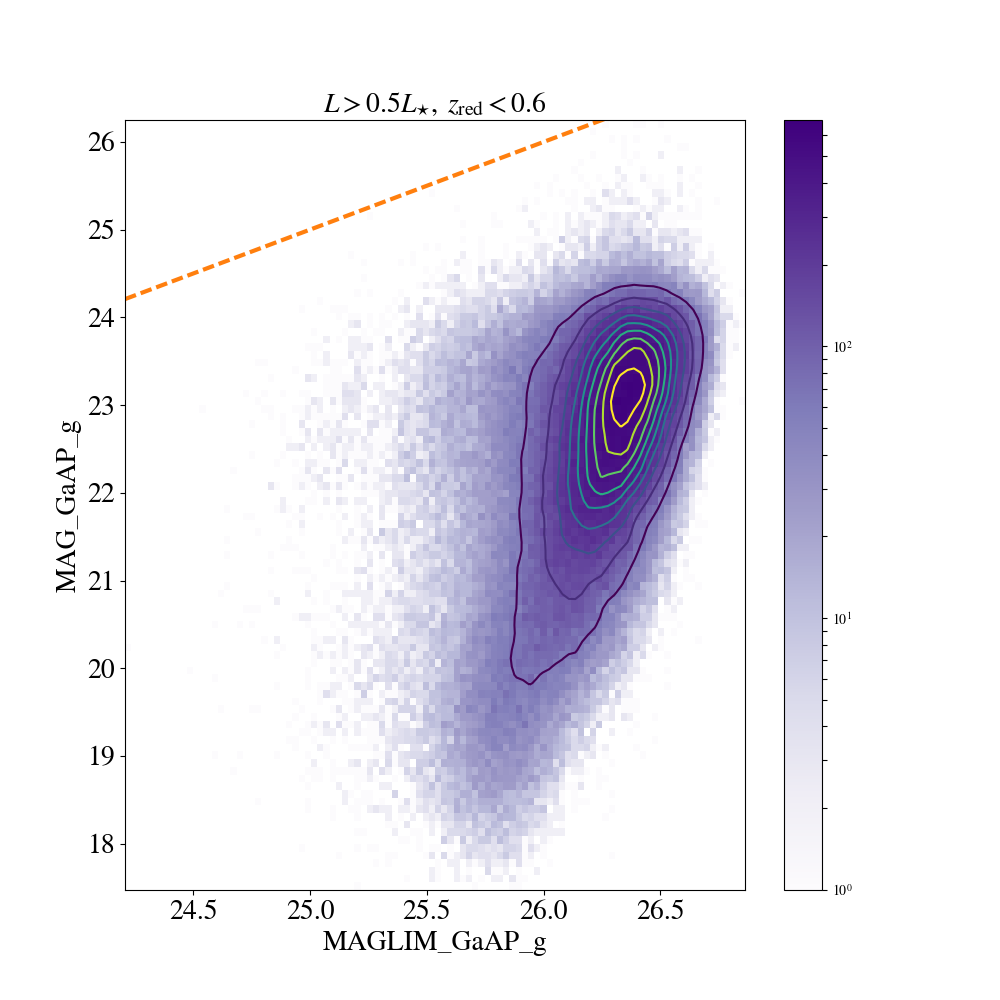
\includegraphics[width=0.5\textwidth]{figures_tmp/magg_lim_type_dense_zmax_0_6.png}
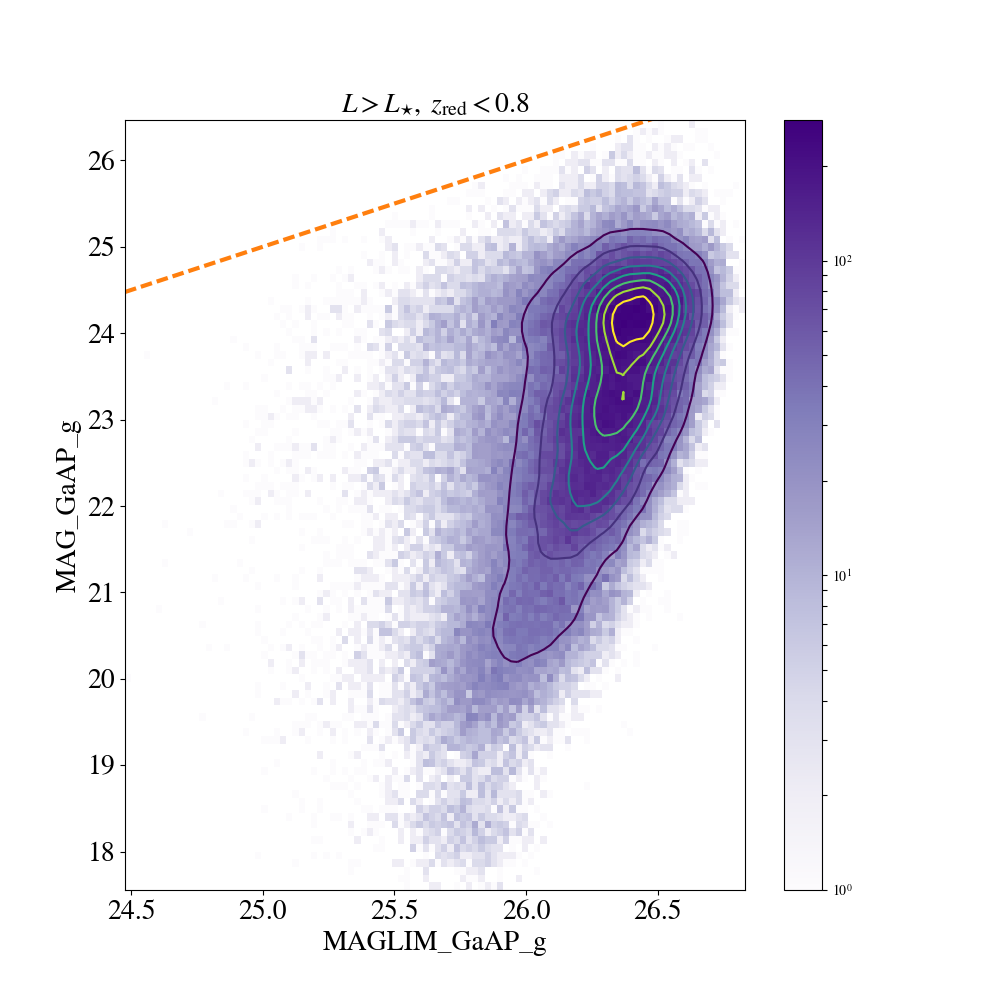
\includegraphics[width=0.5\textwidth]{figures_tmp/magg_lim_type_lum_zmax_0_8.png}
\end{tabular}
\caption{\label{fig:maglim_g} Demonstration of the distributions of the GaAP magnitudes and the limiting magnitudes in the $g$-band for the dense sample (left panel) and the luminous sample (right panel). In both figures the pixellized distributions and countours are color-coded by the number counts. Note that the maximum redshifts of the two samples, $z_{\rm red}=0.6$ (dense) sample and $z_{\rm red}=0.8$ (luminous) sample are chosen such that the samples remain volume-limited and not limited by the varying depth of the survey (showin with the dashed orange line in both panels).} 
\end{figure*}

\begin{figure}
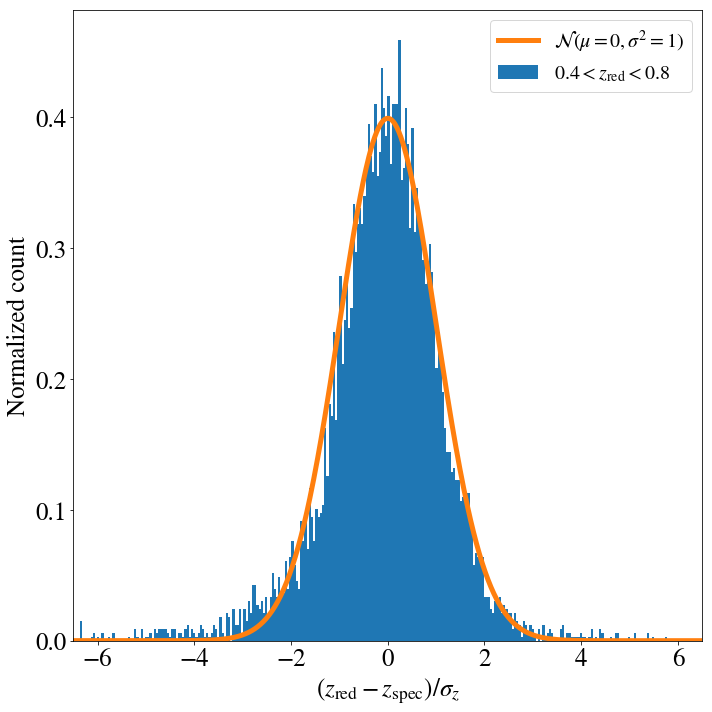
\includegraphics[width=\columnwidth]{figures_tmp/zerr_dist_2.png}
\caption{\label{fig:pz} The Blue hisogram shows the distribution of the offset between the red-sequence redshifts $z_{\rm red}$ and the spectroscopic redshifts $z_{\rm spec}$, weighted by their corresponding redshift uncertainties $\sigma_{z_{\rm red}}$. The orange solid line is a Gaussian distribution with zero mean and standard deviation of unity. This demonstrates that the a Gaussian distribution is a good description of the red-sequence redshift probability distribution functions of galaxies in the our sample of luminous red galaxies.} 
\end{figure}


\begin{figure*}
 \begin{tabular}{cc}
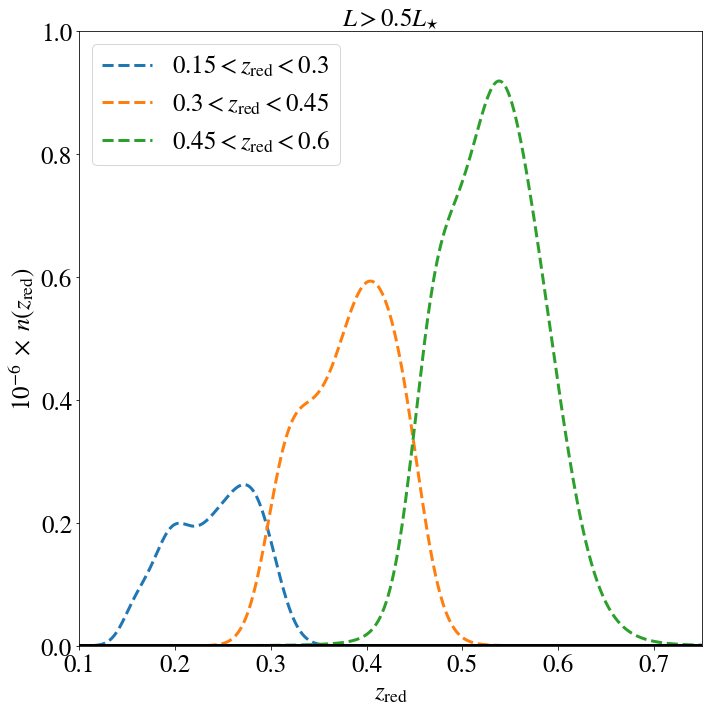
\includegraphics[width=0.4\textwidth]{figures_tmp/nz_dense.png}
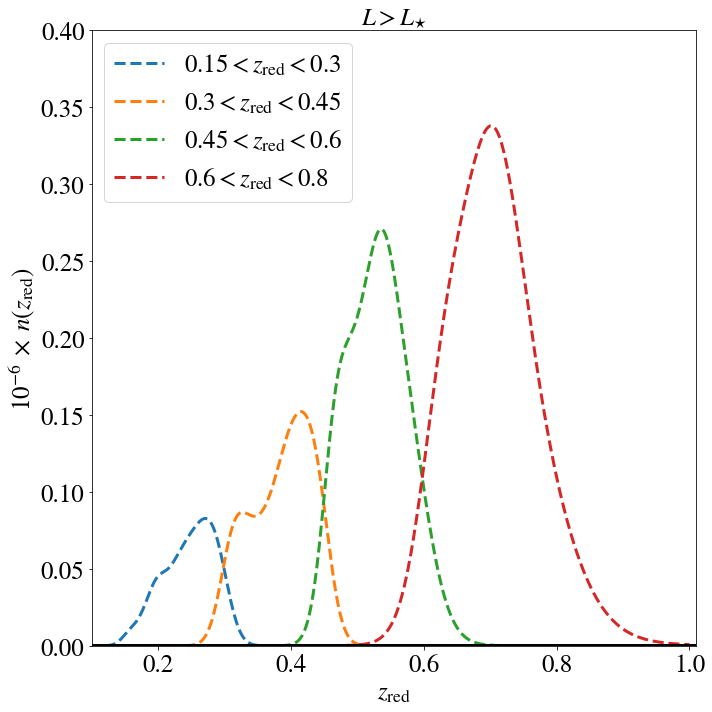
\includegraphics[width=0.4\textwidth]{figures_tmp/nz_lum.png}
\end{tabular}
\caption{\label{fig:nz}  Tomographic redshift distributions of the lens and the source galaxies for the purpose of galaxy-galaxy lensing analysis. The Left and the middle panels show the redshift distributions of the dense and the luminous galaxies respectively. These galaxies are considered as lens galaxies in our lensing analysis. The redshift distributions of the lenses are estimated directly from the the individual red-sequence redshift estimates and their corresponding uncertainties. The right panel shows the redshift distributions of the source galaxies in the KiDS-1000 cosmic shear data. These redshift distributions are estimated from the DIR method taking advantage of the deep spectroscopic calibration fields targeted by KiDS.} 
\end{figure*}




\begin{figure*}
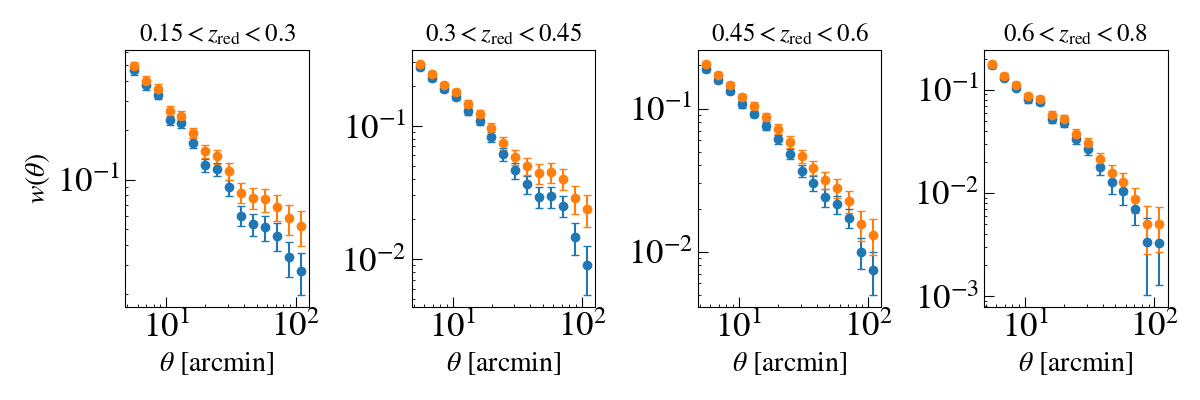
\includegraphics[width=\textwidth]{figures_tmp/xi.png}
\caption{\label{fig:xi} Clustering measurements for the four tomographic bins. In each panel, the blue (orange) data-points correspond to the 2PCF computed using the organized (uniform) randoms.} 
\end{figure*}

\begin{figure*}
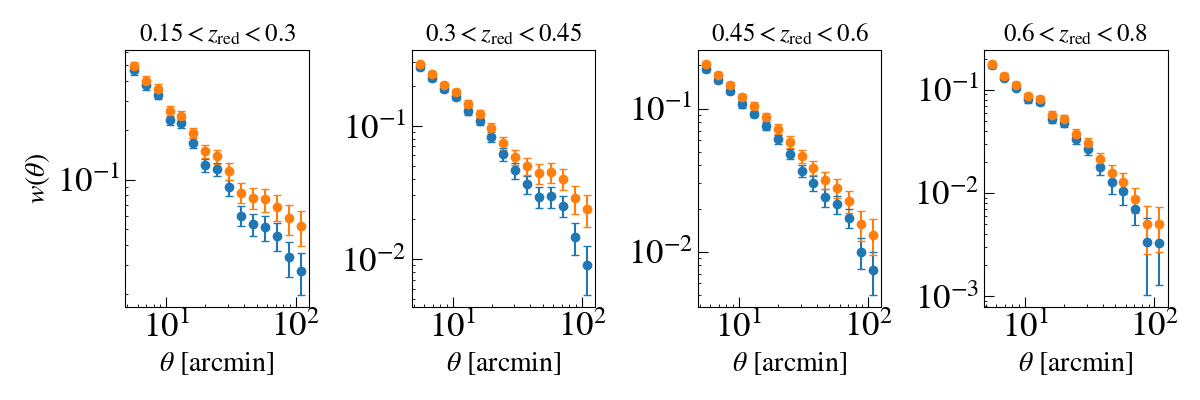
\includegraphics[width=\textwidth]{figures_tmp/xi.png}
\caption{\label{fig:xi} Clustering measurements for the four tomographic bins. In each panel, the blue (orange) data-points correspond to the 2PCF computed using the organized (uniform) randoms.} 
\end{figure*}


%%%%%%%%%%%%%%%%%%%%%%%%%%%%%%%%%%%%%%%%%%%%%%%%%%

%%%%%%%%%%%%%%%%%%%% REFERENCES %%%%%%%%%%%%%%%%%%
% BibTeX:

\bibliographystyle{mnras}
\bibliography{lrg_kids.bib}

%%%%%%%%%%%%%%%%%%%%%%%%%%%%%%%%%%%%%%%%%%%%%%%%%%

%%%%%%%%%%%%%%%%% APPENDICES %%%%%%%%%%%%%%%%%%%%%
%\clearpage

\appendix


\bsp	% typesetting comment
\label{lastpage}
\end{document}
